\chapter{Metodologi}
\label{chap:metodologi}

\section{Metode yang Digunakan}
\label{sec:metode-yang-digunakan}

Penelitian ini menggunakan metode \textit{Federated Learning} pada perangkat \textit{Edge Computing} sebagai pendekatan utama. Secara umum, alur penelitian dari awal hingga akhir ditunjukkan pada Gambar \ref{fig:diagram-alur-penelitian} berikut.

\begin{figure}[H]
  \centering
  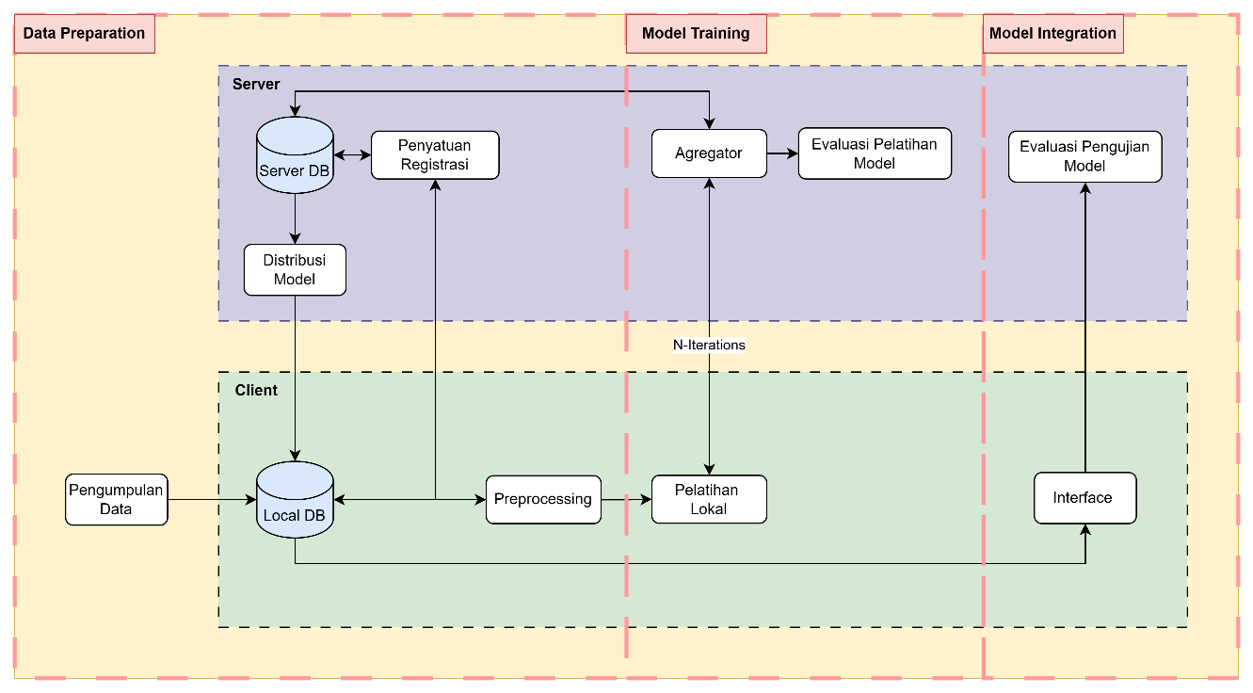
\includegraphics[width=0.8\textwidth]{gambar/Diagram_Alur_Penelitian.png}
  \caption{Diagram Alur Penelitian}
  \label{fig:diagram-alur-penelitian}
\end{figure}

\subsection{\textit{Data Preparation}}
\label{subsec:data-prep}

\begin{enumerate}
  \item \textbf{Pengumpulan Data} \\
  Langkah pertama adalah merekam video wajah dari 30 mahasiswa menggunakan \textit{webcam}. Video tersebut kemudian diekstraksi secara otomatis menjadi kumpulan frame dengan interval pengambilan setiap 0,17 detik, sebagaimana diilustrasikan pada Gambar \ref{fig:sampel-citra-mentah}. Guna mensimulasikan skenario \textit{Federated Learning} yang mendekati kondisi nyata, seluruh data tidak disimpan pada satu lokasi terpusat, melainkan didistribusikan ke beberapa perangkat \textit{edge} sehingga masing-masing perangkat menyimpan data dari 15 mahasiswa yang berbeda.

  \begin{figure}[H]
    \centering
    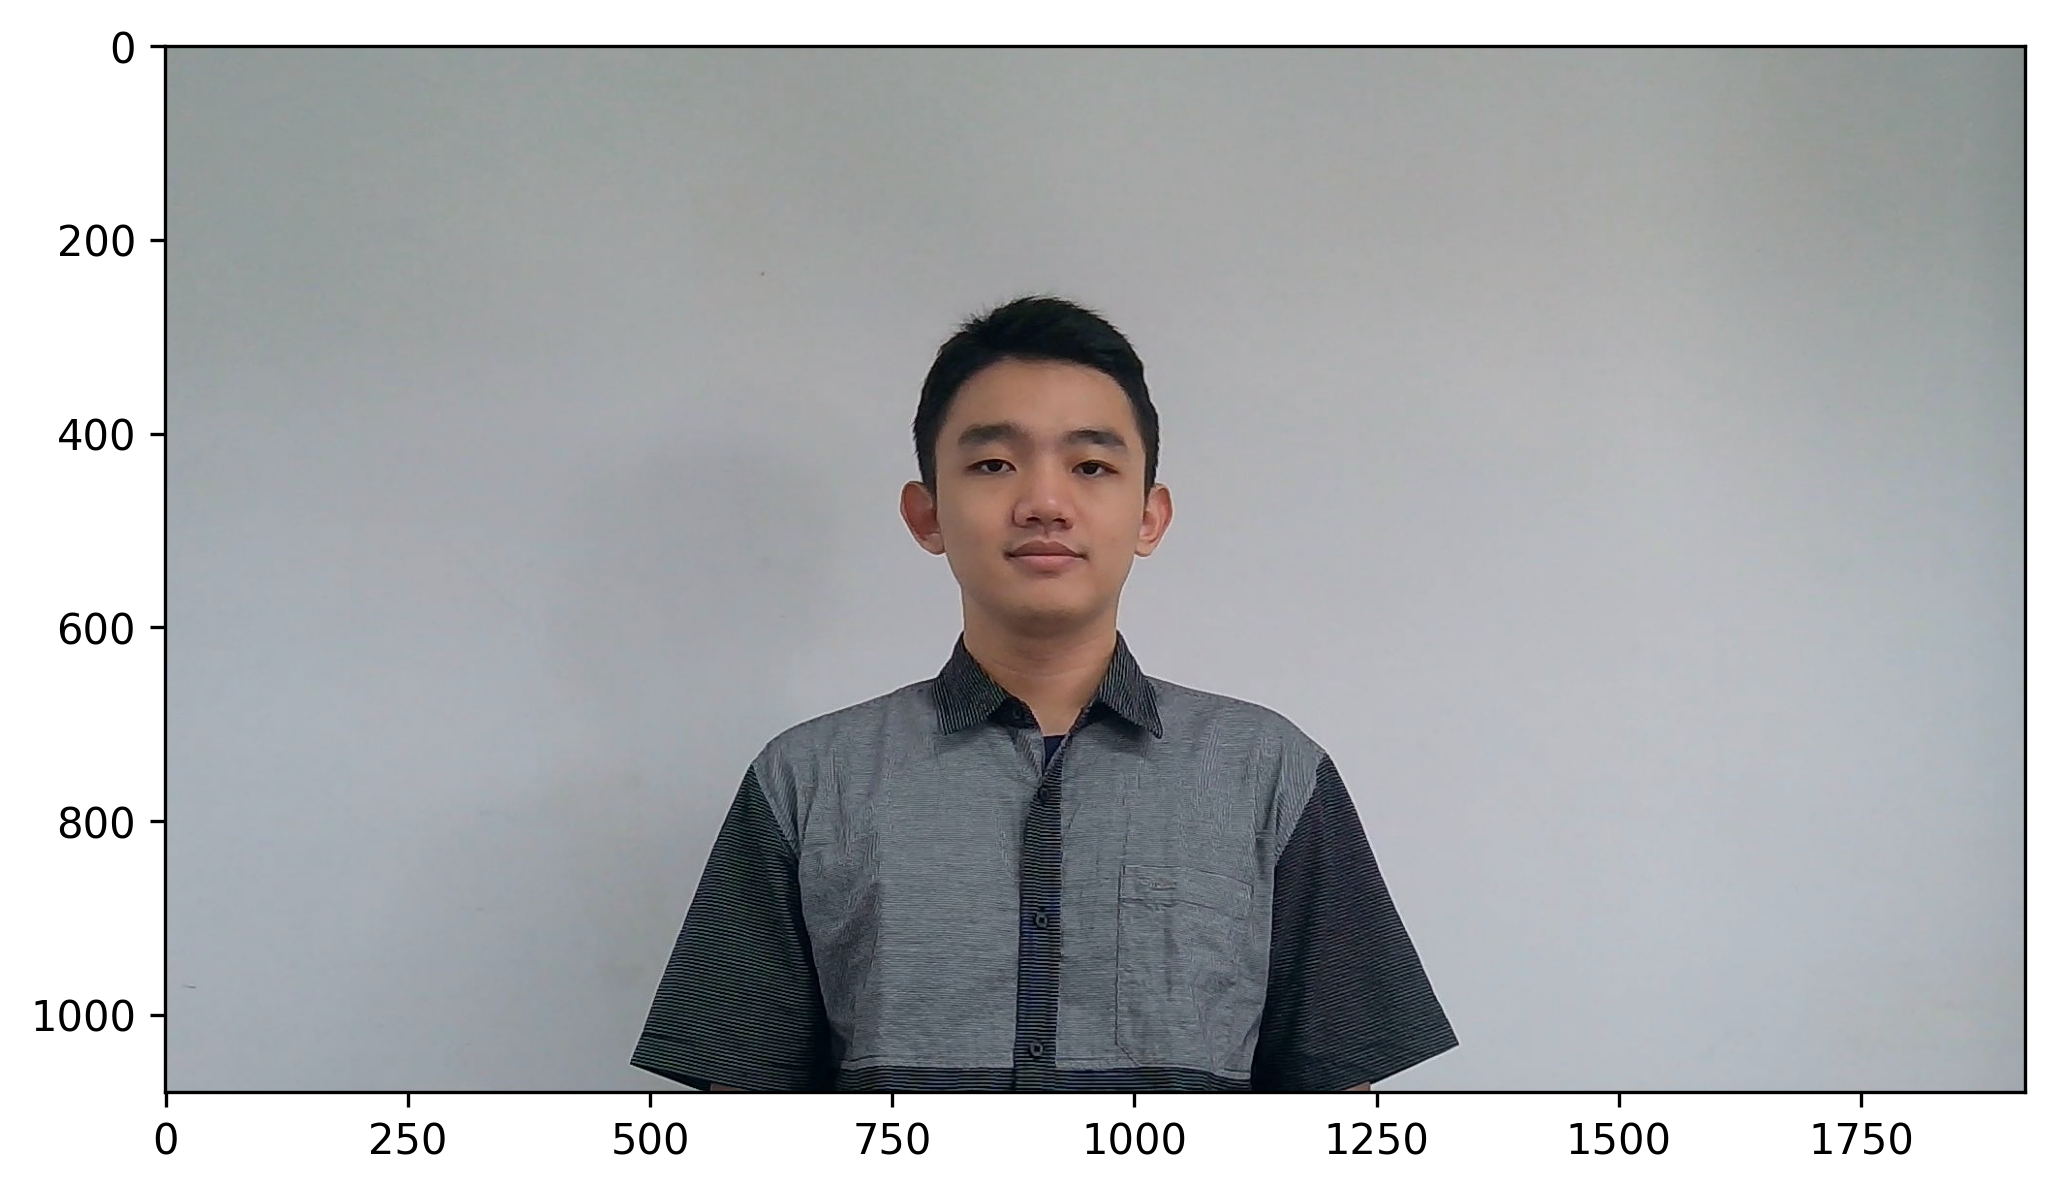
\includegraphics[width=0.8\textwidth]{gambar/1_original_raw.png}
    \caption{Sampel Citra Mentah Hasil Ekstraksi Frame}
    \label{fig:sampel-citra-mentah}
  \end{figure}

  \item \textbf{Distribusi Model} \\
  Setelah data terdistribusi, server mendistribusikan bobot awal model (\textit{pre-trained weights}) ke setiap perangkat \textit{client}. Langkah ini memastikan seluruh perangkat memiliki titik awal yang seragam sebelum masing-masing menjalankan pelatihan lokal menggunakan data 15 mahasiswa yang dikelolanya.

  \item \textbf{Penyatuan Registrasi} \\
  Setiap perangkat \textit{client} mendaftarkan identitas 15 mahasiswanya ke server pusat. Server kemudian menyusun satu daftar label terpadu yang mencakup seluruh 30 mahasiswa sehingga tidak terjadi tumpang tindih penomoran label antar-perangkat. Daftar terpadu ini menjadi acuan utama dalam proses pengelompokan citra pada tahap \textit{preprocessing}.

  \item \textbf{Preprocessing} \\
  Berdasarkan daftar label yang telah terbentuk, setiap citra wajah diproses secara sekuensial untuk memenuhi format masukan model. Tahapannya adalah sebagai berikut.
  \begin{enumerate}
    \item \textit{Seleksi Laplacian Variance}: Sistem mengukur ketajaman setiap frame menggunakan operator Laplacian yang bekerja dengan mendeteksi gradien tepi objek dalam citra. Frame yang memiliki nilai ketajaman rendah akibat gerakan subjek maupun kondisi pencahayaan yang kurang optimal akan disaring secara otomatis. Dari seluruh frame yang tersedia, dipilih 50 frame dengan nilai ketajaman tertinggi untuk diteruskan ke tahap berikutnya. Perbandingan visual antara citra tajam dan citra buram dapat dilihat pada Gambar \ref{fig:laplacian-variance}.

    \begin{figure}[H]
      \centering
      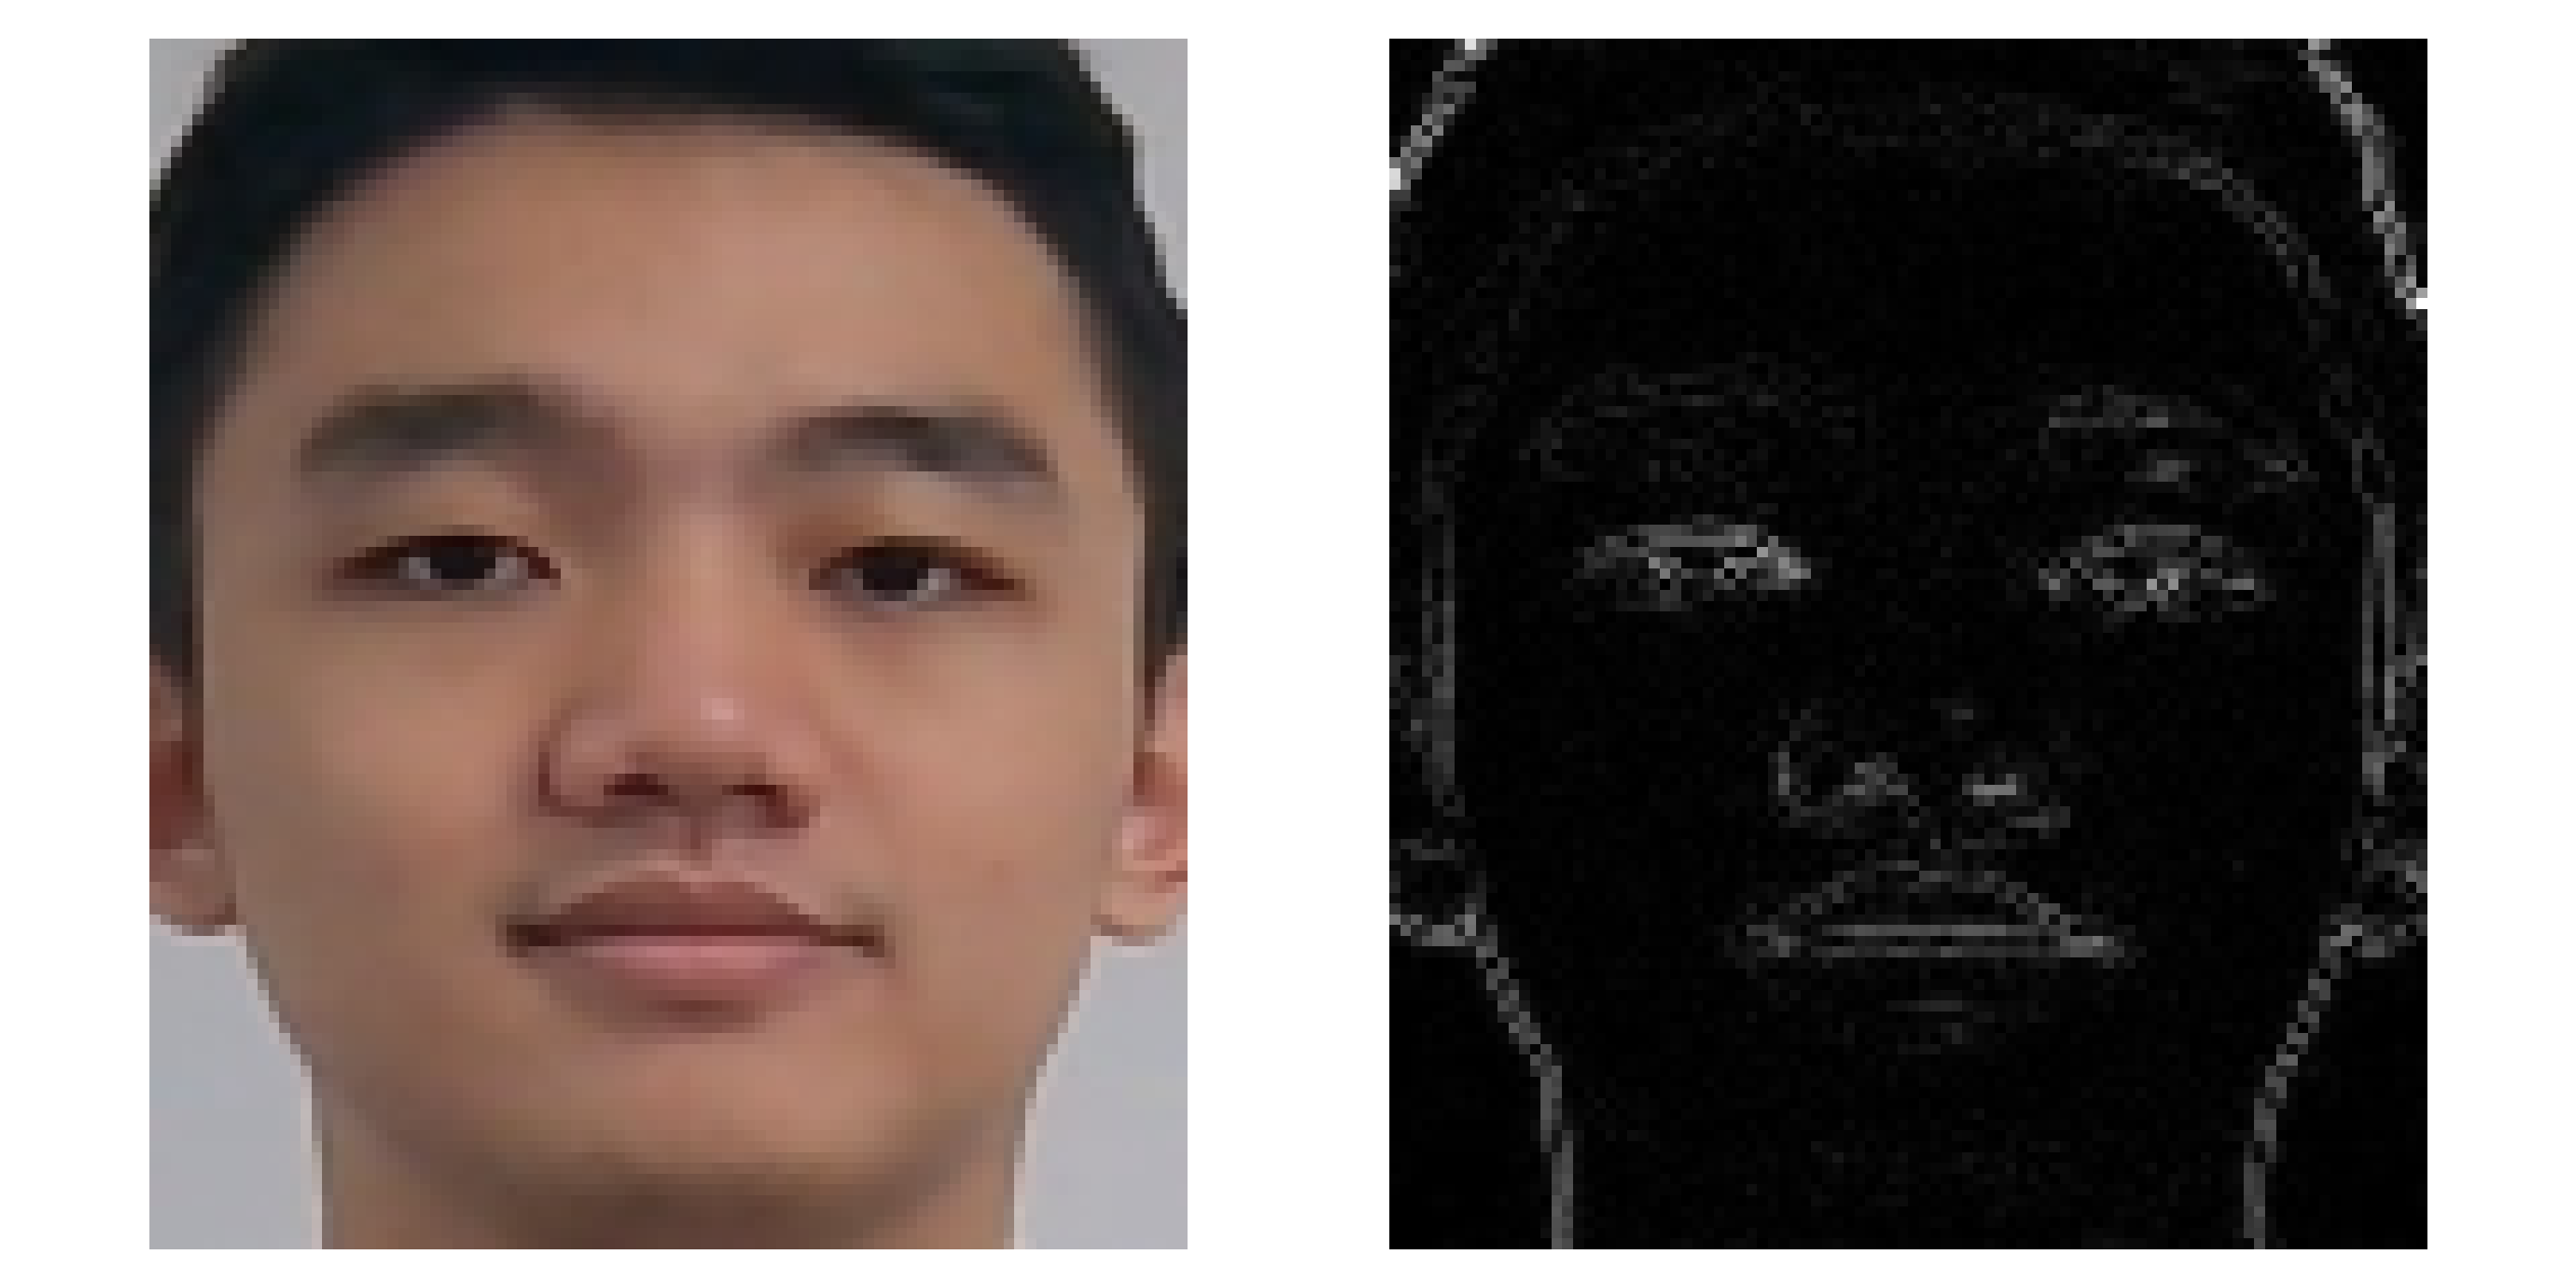
\includegraphics[width=0.8\textwidth]{gambar/2_laplacian_sharpness.png}
      \caption{Hasil Penyaringan Ketajaman Citra Menggunakan Laplacian Variance}
      \label{fig:laplacian-variance}
    \end{figure}

    \item \textit{Face Detection dan Cropping}: Dari 50 frame terpilih, model MTCNN melokalisasi wajah secara otomatis dengan menghasilkan koordinat kotak pembatas di sekitar area wajah sekaligus mengekstraksi posisi 5 titik penanda wajah, yaitu mata kiri, mata kanan, hidung, sudut mulut kiri, dan sudut mulut kanan. Koordinat tersebut digunakan untuk memotong citra secara presisi sehingga hanya area wajah yang dipertahankan, sebagaimana ditunjukkan pada Gambar \ref{fig:mtcnn-detection}.

    \begin{figure}[H]
      \centering
      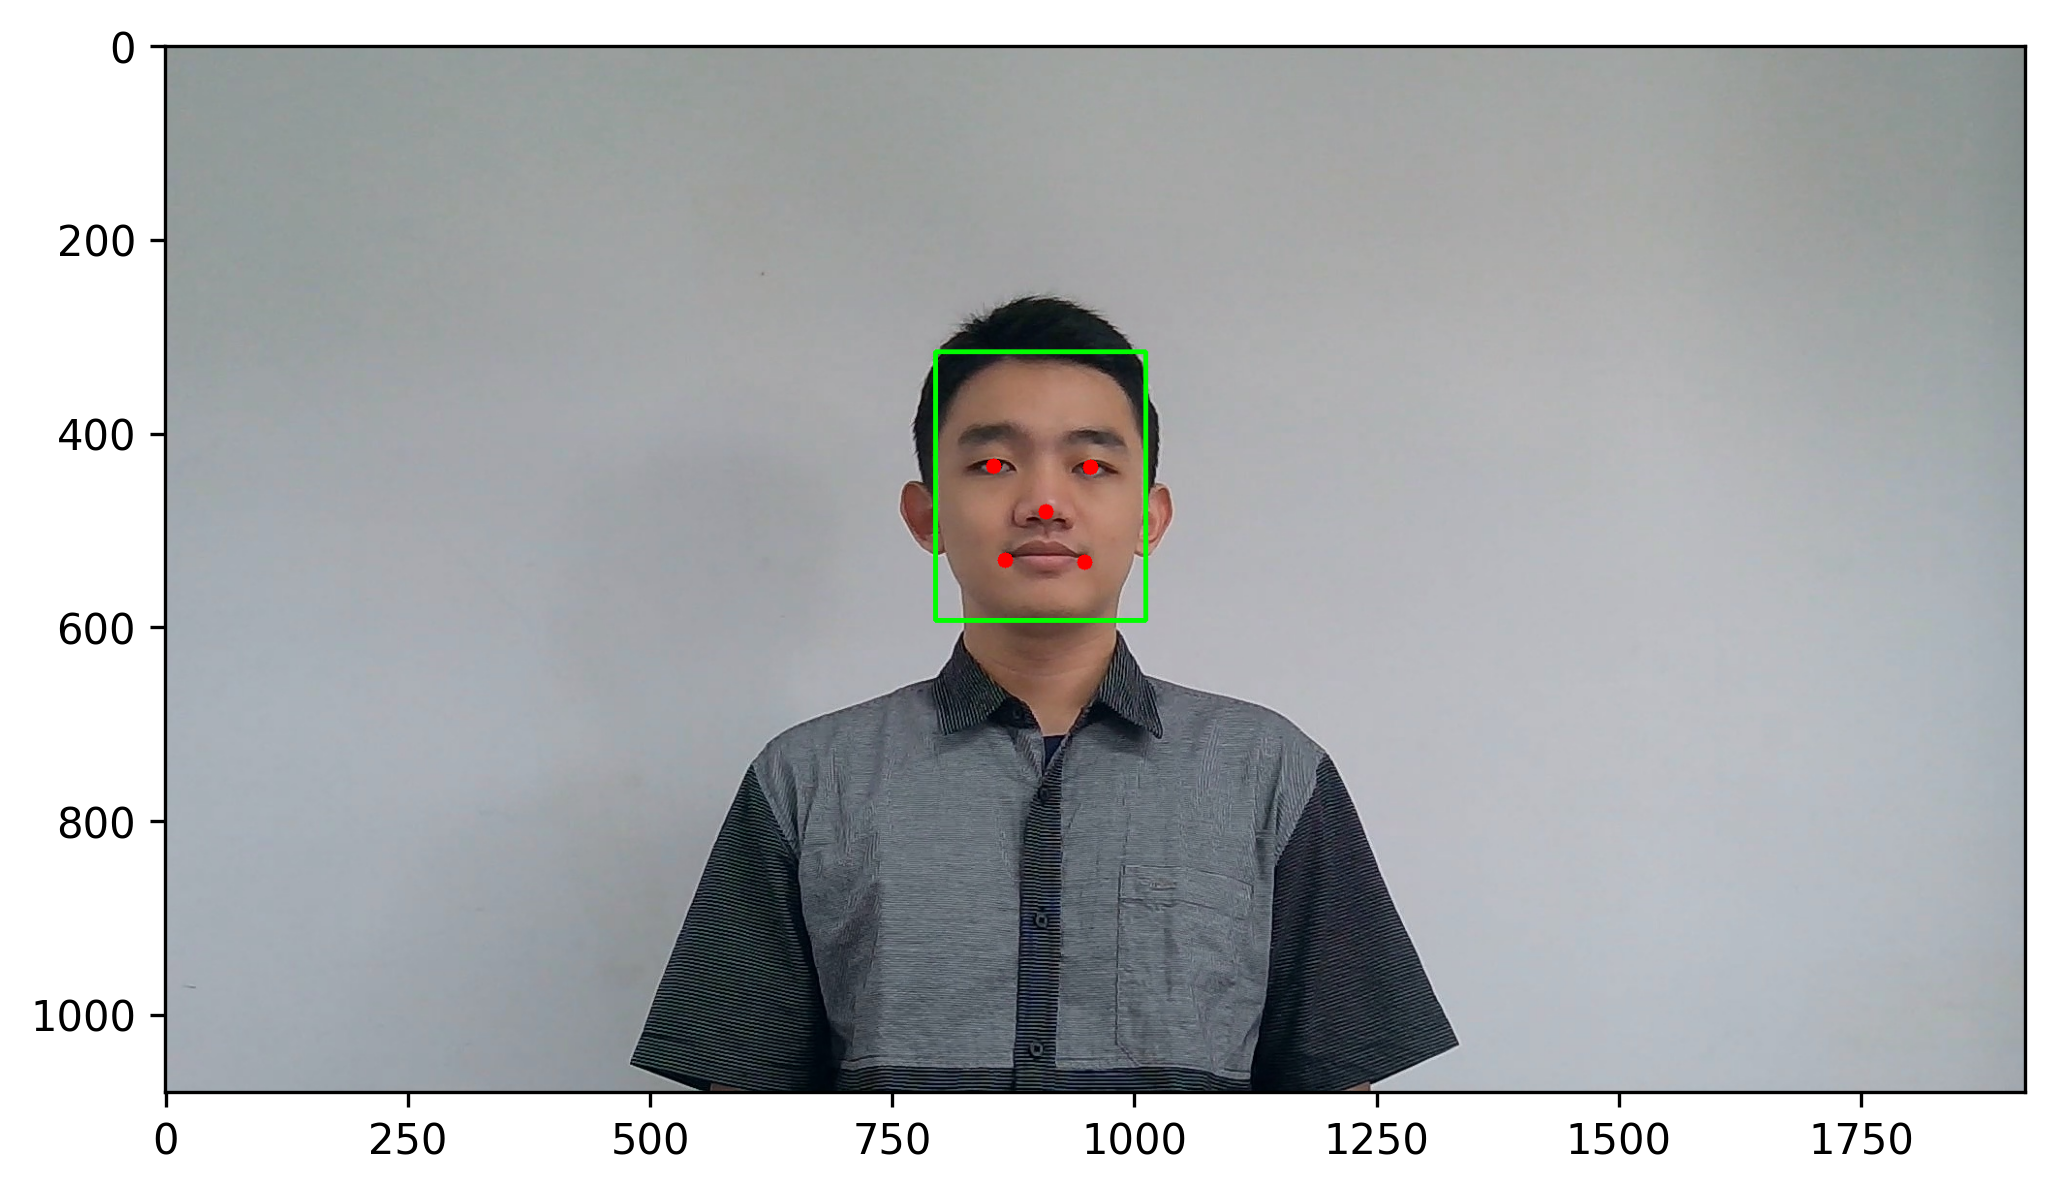
\includegraphics[width=0.8\textwidth]{gambar/3_mtcnn_detection.png}
      \caption{Deteksi Bounding Box dan Titik Landmarks Wajah Menggunakan MTCNN}
      \label{fig:mtcnn-detection}
    \end{figure}

    \item \textit{Resizing}: Citra wajah hasil pemotongan diubah ukurannya menjadi 96$\times$112 piksel karena arsitektur MobileFaceNet hanya dapat menerima citra dengan dimensi tersebut sebagai masukan lapisan konvolusi pertamanya. Hasil normalisasi resolusi ini dapat dilihat pada Gambar \ref{fig:normalisasi-resolusi}.

    \begin{figure}[H]
      \centering
      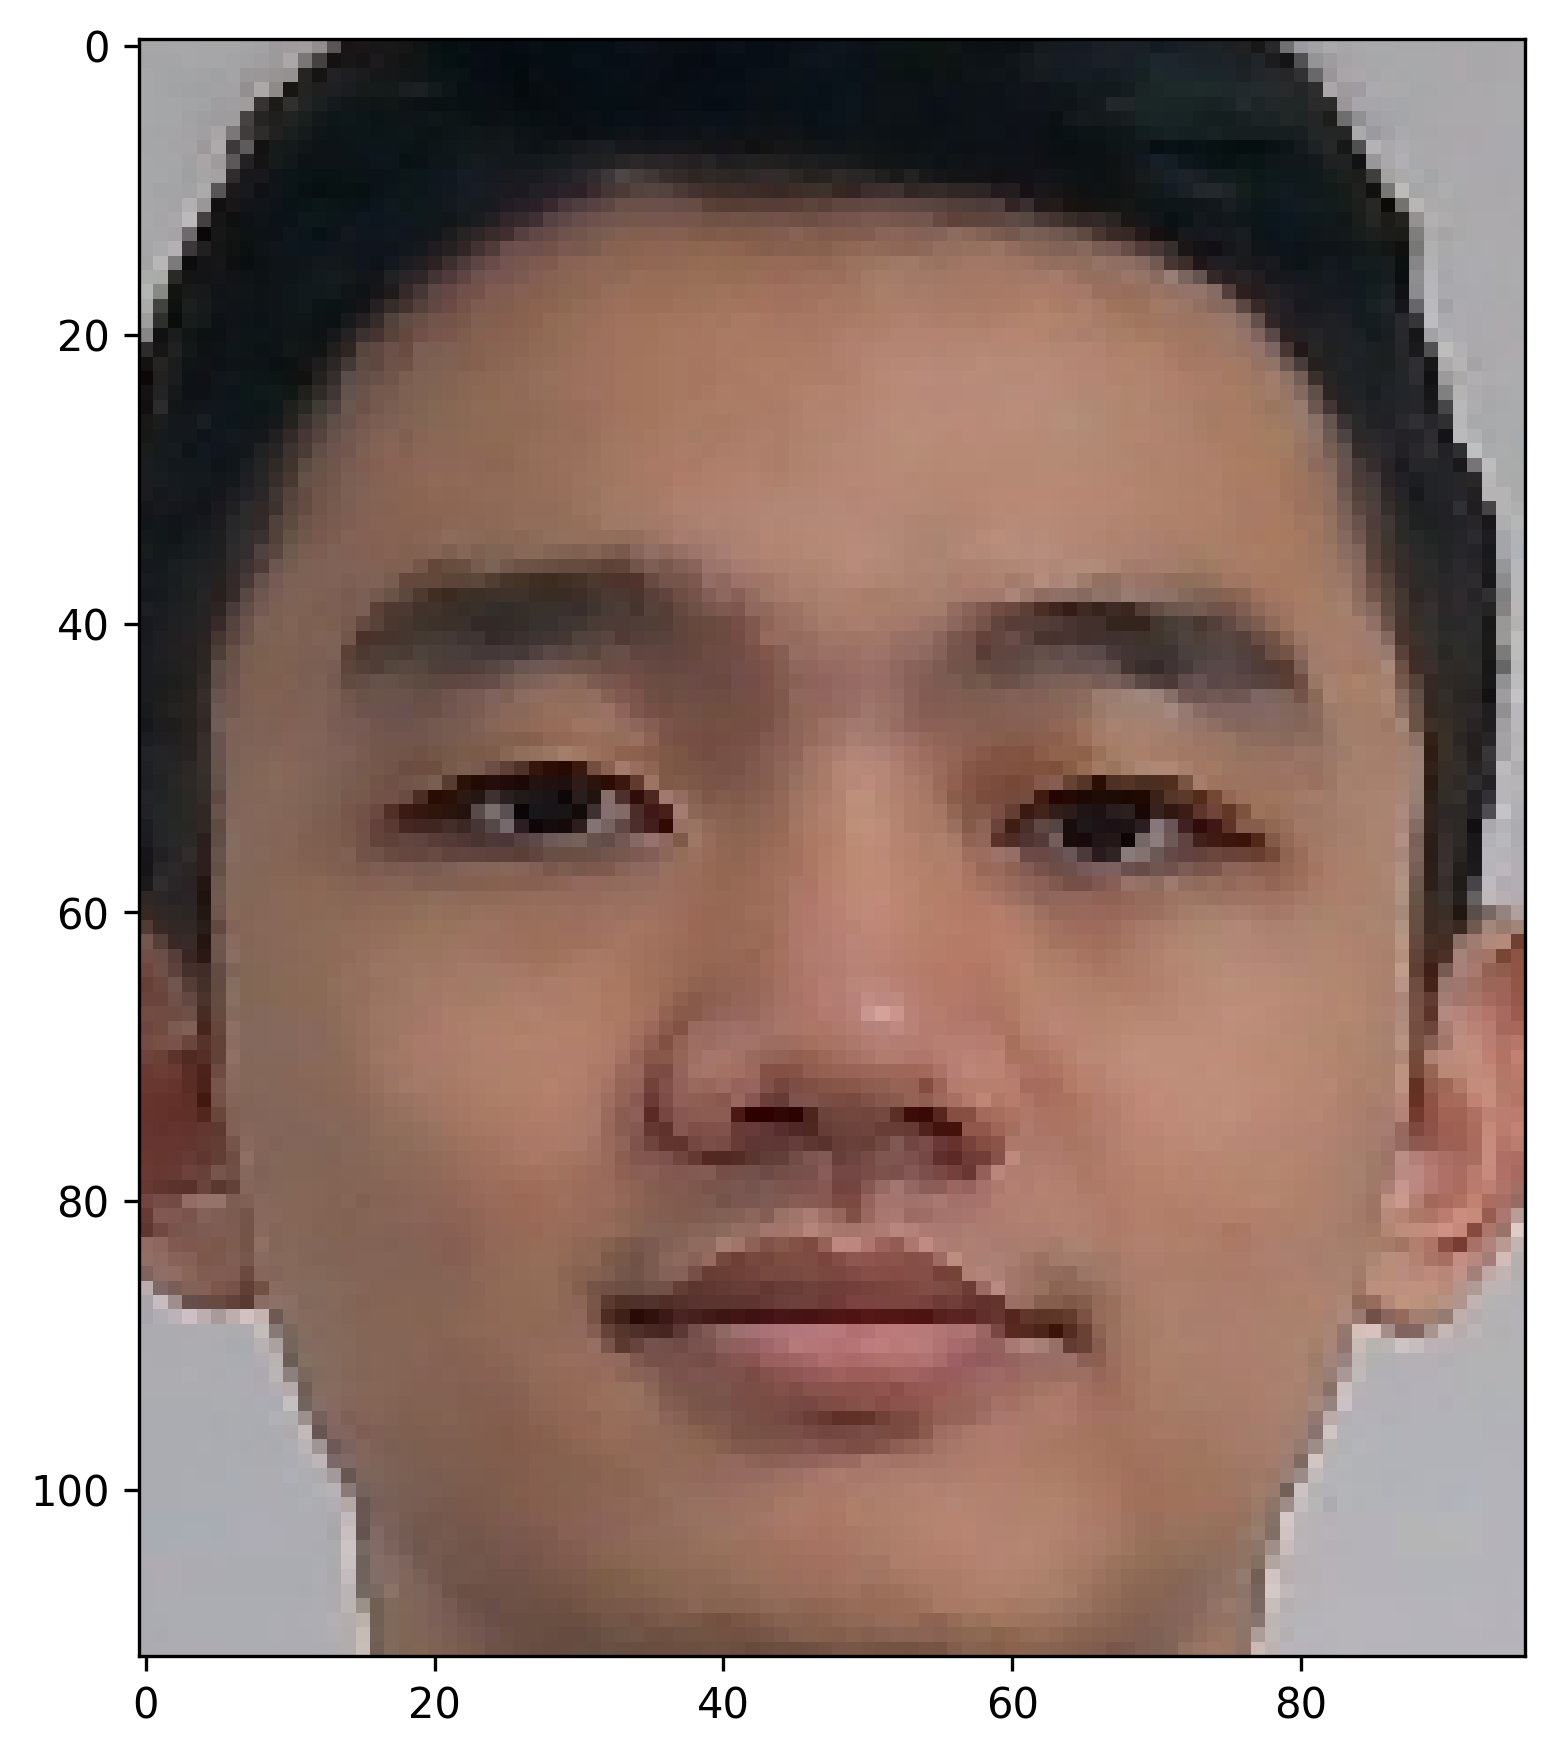
\includegraphics[width=0.8\textwidth]{gambar/4_aligned_face.png}
      \caption{Hasil Normalisasi Citra Wajah Menjadi Resolusi 96x112 Piksel}
      \label{fig:normalisasi-resolusi}
    \end{figure}

    \item \textit{Normalization}: Nilai piksel citra dinormalisasi agar berada pada rentang yang konsisten. Citra dikonversi ke format \textit{tensor} multidimensi, kemudian setiap nilai piksel dikurangi nilai rata-rata sebesar 0,5 dan dibagi dengan standar deviasi sebesar 0,5. Normalisasi ini bertujuan menstabilkan distribusi gradien sehingga proses pelatihan model berlangsung lebih stabil dan konvergen lebih cepat.

    \item \textit{Enkripsi}: Vektor \textit{face embedding} yang dihasilkan model dienkripsi sebelum disimpan ke database lokal menggunakan algoritma AES-256 dalam mode CBC. Dengan demikian, meskipun perangkat \textit{edge} berhasil diakses secara fisik oleh pihak tidak berwenang, data biometrik yang tersimpan tidak dapat dibaca maupun direkonstruksi kembali tanpa kunci enkripsi yang valid.
  \end{enumerate}
\end{enumerate}

\subsection{\textit{Model Training}}
\label{subsec:model-training-alur}

Proses pelatihan dimulai setelah semua citra wajah di setiap perangkat \textit{edge} selesai dibersihkan, dipotong, dan diamankan. Tujuan dari tahap ini adalah melatih model MobileFaceNet secara kolaboratif agar mampu mengenali wajah mahasiswa tanpa harus mengirimkan data ke server. Proses ini berjalan berulang dalam beberapa ronde menggunakan algoritma FedProx dengan langkah-langkah sebagai berikut.

\begin{enumerate}
  \item \textbf{Pelatihan Lokal} \\
  Tahap ini merupakan fase komputasi mandiri di sisi perangkat \textit{client} menggunakan data lokal terisolasi dari 15 mahasiswa yang dikelolanya. Alurnya dibagi ke dalam sub-proses berikut.
  \begin{enumerate}
    \item \textit{Konfigurasi Layer Freezing}: Sebelum pelatihan dimulai, sebagian lapisan awal \textit{backbone} MobileFaceNet dibekukan sehingga parameternya tidak ikut diperbarui selama pelatihan. Pembekuan ini menonaktifkan kalkulasi gradien pada lapisan-lapisan terkait, yang secara langsung mengurangi konsumsi memori komputasi pada perangkat \textit{edge}. Dari total 19 lapisan utama MobileFaceNet yang terdiri dari 1 lapisan konvolusi awal, 1 konvolusi depthwise, dan 17 blok \textit{bottleneck}, sistem membekukan 14 lapisan pertama. Lapisan yang tetap aktif dan dilatih meliputi 5 blok \textit{bottleneck} terakhir, lapisan \textit{embedding}, serta lapisan klasifikasi. Skema ini diterapkan karena keterbatasan kapasitas RAM pada perangkat \textit{edge} seperti Raspberry Pi tidak memungkinkan pelatihan penuh seluruh lapisan secara serentak.

    \item \textit{Augmentasi Data On-The-Fly}: Setiap citra wajah dimodifikasi secara acak pada saat pemuatan data tanpa mengubah berkas aslinya di penyimpanan fisik. Teknik augmentasi yang diterapkan meliputi pembalikan horizontal acak untuk mensimulasikan variasi sudut pandang wajah, perubahan acak kecerahan dan kontras untuk meniru fluktuasi intensitas cahaya ruangan, rotasi acak untuk mensimulasikan kemiringan kepala subjek, pemotongan dan penskalaan ulang acak untuk mensimulasikan variasi jarak terhadap kamera, serta konversi ke skala abu-abu secara acak untuk melatih ketahanan ekstraksi fitur pada kondisi minim warna. Variasi citra hasil augmentasi ini ditunjukkan pada Gambar \ref{fig:data-augmentation}.

    \begin{figure}[H]
      \centering
      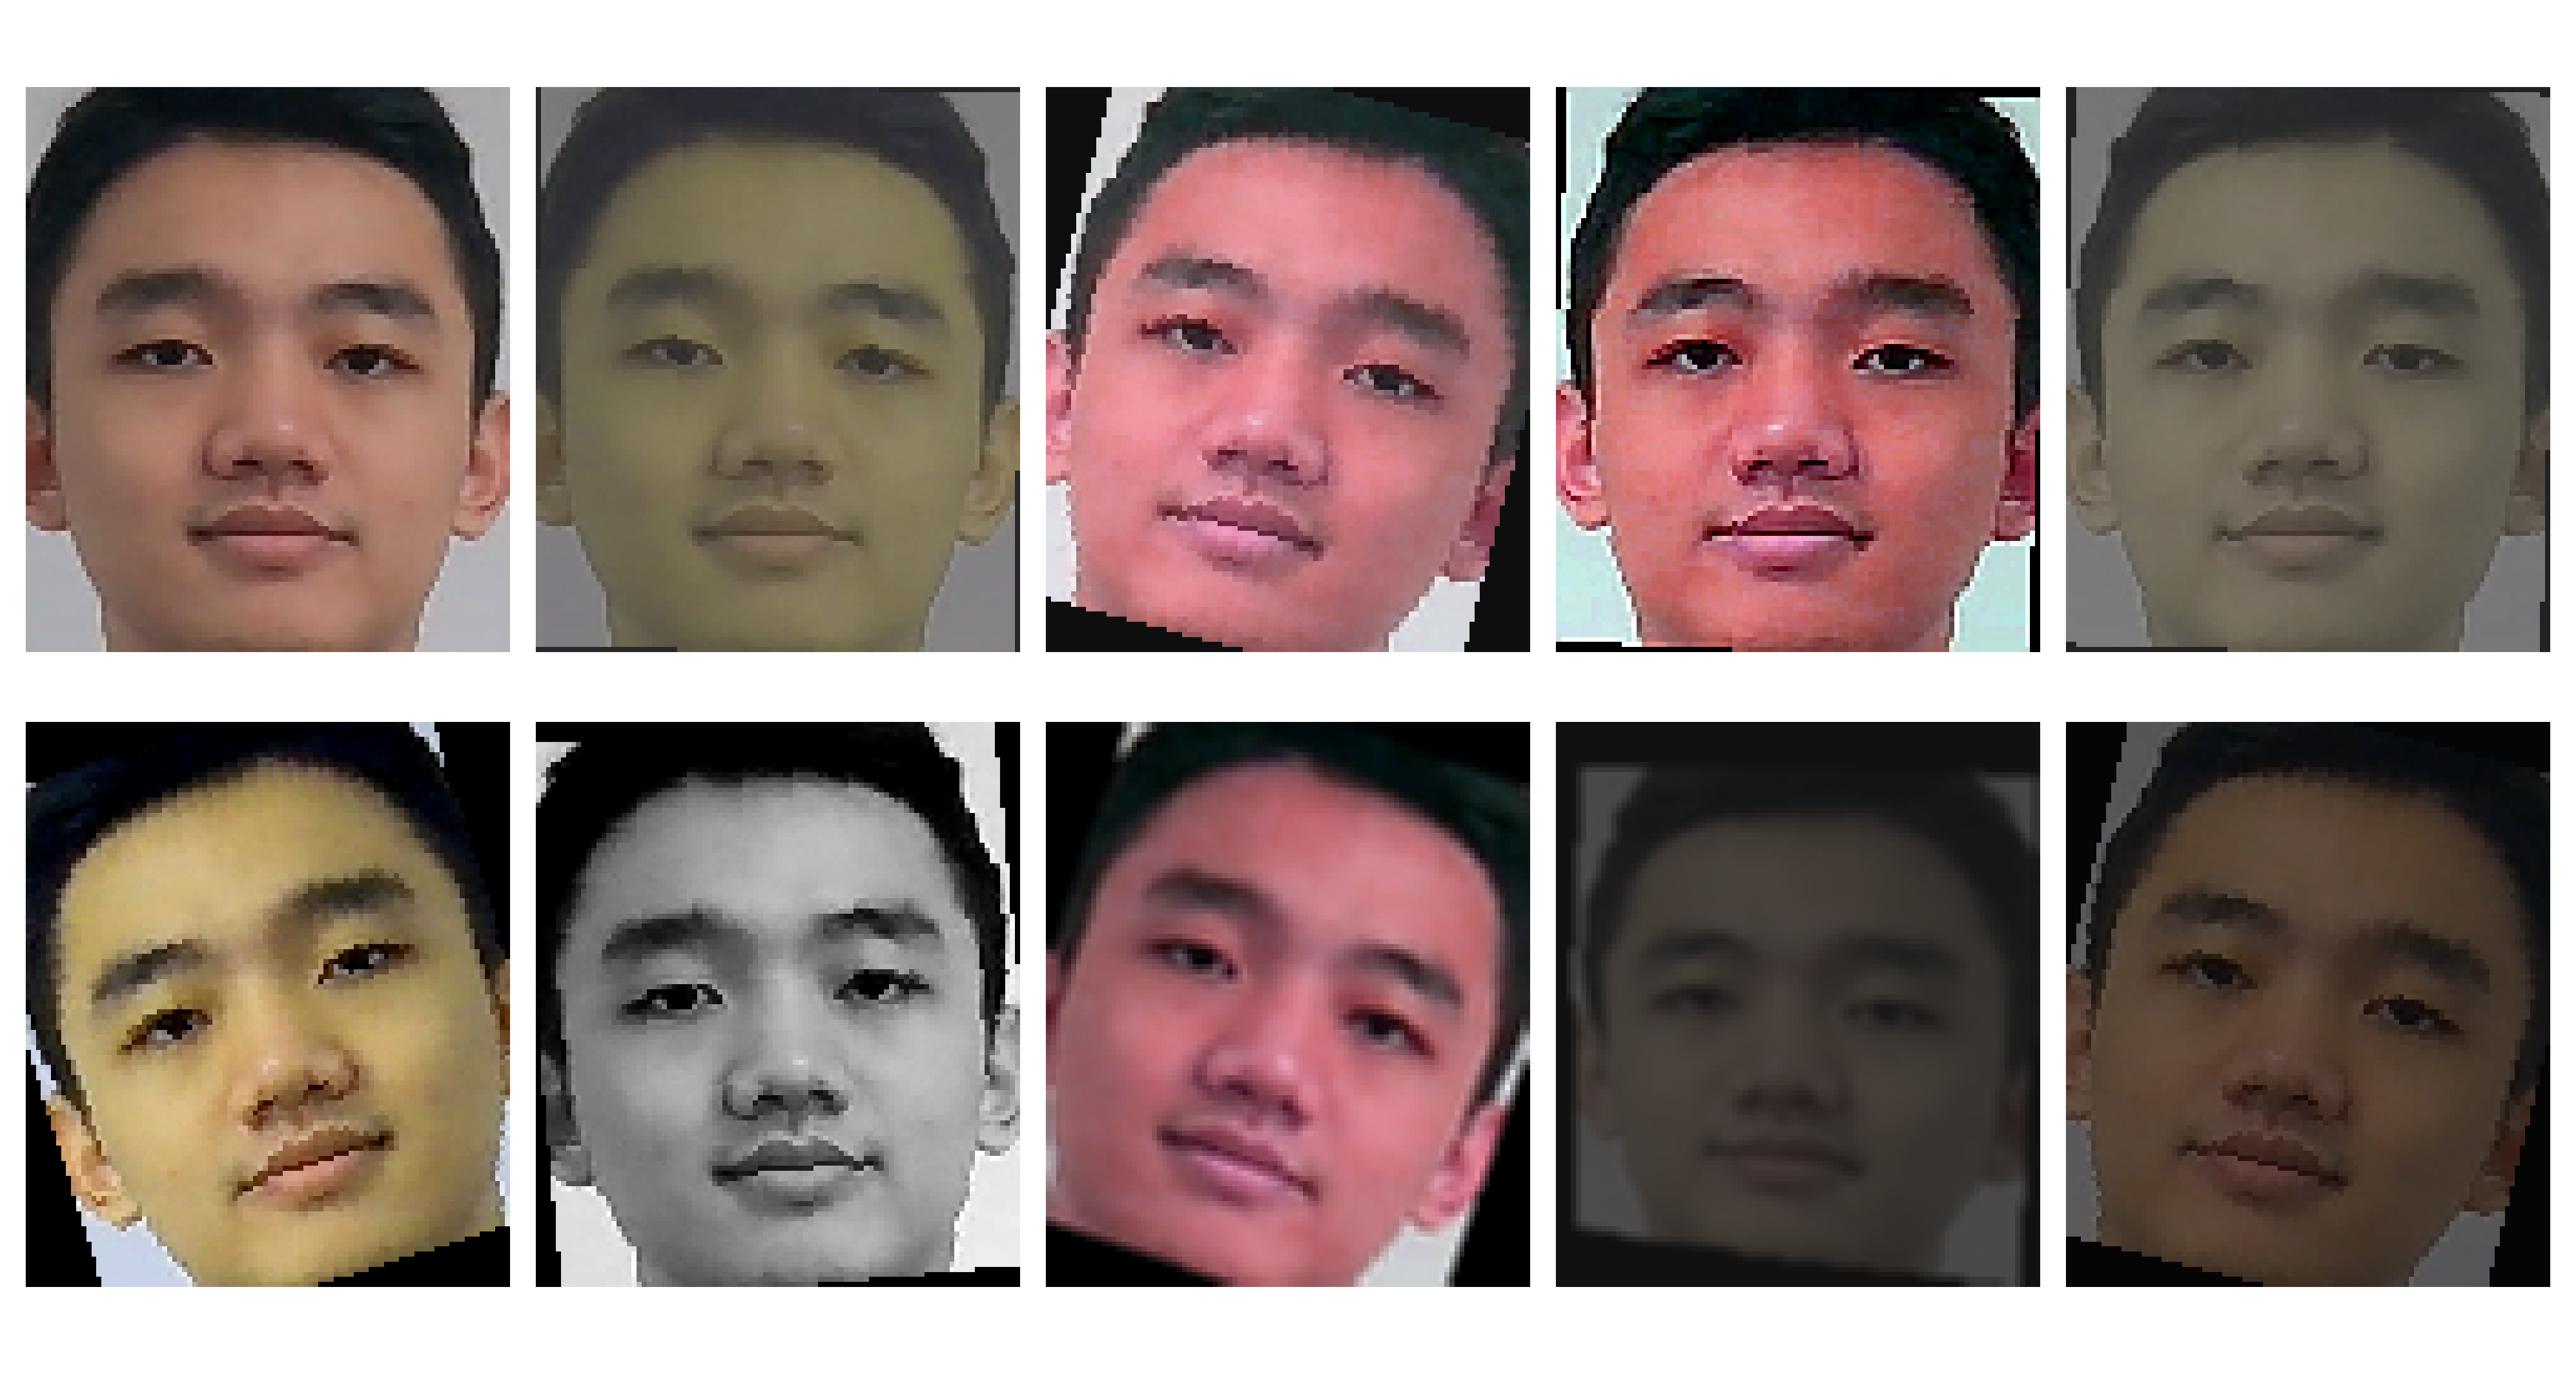
\includegraphics[width=0.8\textwidth]{gambar/5_augmentation_samples.png}
      \caption{Variasi Sampel Hasil Transformasi On-the-Fly Data Augmentation}
      \label{fig:data-augmentation}
    \end{figure}

    \item \textit{Hiperparameter dan Optimasi Lokal dengan FedProx Proximal Term}: Pelatihan lokal pada setiap perangkat \textit{client} dikonfigurasi dengan beberapa parameter utama. Algoritma optimasi yang digunakan adalah \textit{Stochastic Gradient Descent} (SGD) dengan nilai momentum 0,9 dan Nesterov diaktifkan untuk mempercepat konvergensi dan menstabilkan pembaruan bobot. Setiap ronde, model dilatih selama 1 \textit{epoch} dengan ukuran \textit{batch} 32. Laju pembelajaran (\textit{learning rate}) dimulai dari 0,01 dan diturunkan secara bertahap mengikuti pola \textit{Cosine Decay}. Fungsi kerugian yang diterapkan adalah \textit{ArcFace Margin Loss} yang dirancang khusus untuk pengenalan wajah dengan mempertegas separasi antar kelas dalam ruang fitur. Di samping itu, ditambahkan komponen penalti \textit{Proximal Term} dengan nilai $\mu = 0{,}05$ dari algoritma FedProx yang berfungsi membatasi deviasi parameter model lokal terhadap model global acuan. Penalti ini penting dalam skenario distribusi data yang tidak merata antar-perangkat karena tanpa mekanisme ini model pada setiap \textit{client} berpotensi berkembang ke arah yang divergen sehingga sulit diagregasikan.

    \item \textit{Ekstraksi Parameter dan Head Centroid}: Setelah satu ronde pelatihan lokal selesai, sistem mengambil dua komponen dari model, yaitu bobot lapisan konvolusi yang sudah diperbarui dan \textit{head centroid weights} yang merepresentasikan profil rata-rata setiap identitas mahasiswa di lapisan klasifikasi. Kedua komponen ini dikemas menjadi satu paket data yang siap dikirim ke server.

    \item \textit{Transmisi Parameter}: Paket parameter tersebut dikirimkan ke server pusat melalui jaringan lokal. Yang ditransmisikan hanyalah nilai bobot model hasil pelatihan, bukan citra wajah mahasiswa dalam bentuk apapun. Mekanisme ini menjamin bahwa data biometrik asli tetap tersimpan secara eksklusif di dalam perangkat \textit{edge} sepanjang siklus komunikasi berlangsung.
  \end{enumerate}

  \item \textbf{Aggregator} \\
  Setelah semua \textit{client} mengirimkan hasil pelatihan lokalnya, server bertugas menggabungkan seluruh parameter tersebut menjadi satu model global. Proses ini terdiri dari tiga langkah berikut.
  \begin{enumerate}
    \item \textit{Pengumpulan Parameter}: Server mengumpulkan semua bobot model dan \textit{head centroid weights} dari setiap \textit{client} yang aktif pada ronde tersebut, lalu menyelaraskan strukturnya berdasarkan indeks label yang sudah disepakati bersama.
    \item \textit{Penggabungan (Agregasi)}: Server menghitung rata-rata tertimbang dari seluruh bobot yang diterima. \textit{Client} dengan volume data latih lebih besar memperoleh bobot kontribusi yang lebih besar dalam perhitungan. Hasilnya adalah satu model global baru yang memiliki representasi fitur biometrik dari seluruh 30 mahasiswa secara kolektif tanpa sekalipun menerima citra wajah dari perangkat manapun.
    \item \textit{Distribusi Model Global}: Model global yang baru disebarkan kembali ke semua \textit{client} sebagai titik awal pelatihan ronde berikutnya. Siklus ini terus berulang hingga jumlah ronde yang ditargetkan tercapai.
  \end{enumerate}

  \item \textbf{Evaluasi Pelatihan Model} \\
  Untuk mengetahui seberapa baik sistem bekerja, model hasil \textit{Federated Learning} dibandingkan dengan model yang dilatih secara terpusat (\textit{Centralized Learning}) sebagai patokan. Perbandingan dilakukan dari dua sisi.
  \begin{enumerate}
    \item \textit{Evaluasi Performa Pelatihan}: Setiap ronde pelatihan, nilai \textit{loss} dan akurasi pada data latih maupun validasi dicatat ke dalam tabel. Dari tabel ini dapat dilihat apakah model semakin baik dalam mengenali wajah dari ronde ke ronde serta seberapa stabil proses belajarnya.
    \item \textit{Evaluasi Efisiensi Sumber Daya}: Selain akurasi, penelitian ini juga mengukur biaya komputasi yang dikeluarkan, yaitu durasi pelatihan dalam satuan detik, volume data yang dikirim melalui jaringan dalam satuan MB, serta konsumsi energi listrik dalam satuan kWh. Ketiga nilai ini dicatat dan dibandingkan antara kedua pendekatan.
  \end{enumerate}
\end{enumerate}

\subsection{\textit{Model Integration}}
\label{subsec:model-integration-alur}

Tahap \textit{model integration} adalah fase terakhir dari perancangan sistem, di mana model MobileFaceNet yang sudah terlatih diintegrasikan ke dalam aplikasi absensi untuk melakukan pengenalan wajah secara langsung di perangkat \textit{edge}. Tahap ini terbagi menjadi 2 bagian utama.

\begin{enumerate}
  \item \textbf{\textit{Interface}} \\
  Subsistem ini menangani proses absensi secara langsung. Siklus kerjanya dimulai ketika kamera \textit{webcam} aktif dan mulai menangkap video wajah mahasiswa. Setiap frame dari video tersebut dideteksi wajahnya menggunakan MTCNN, lalu diekstraksi karakteristiknya oleh MobileFaceNet menjadi sebuah \textit{face embedding}. Selanjutnya, sistem menghitung seberapa mirip \textit{embedding} tersebut dengan data wajah yang sudah tersimpan di database menggunakan \textit{Cosine Similarity}. Agar tidak salah dalam mengenali identitas akibat gerakan sesaat, sistem menggunakan \textit{Temporal Voting} dengan mengakumulasikan skor kemiripan dari 3 frame terakhir sebelum memutuskan identitas akhir, apakah mahasiswa tersebut dikenal beserta NRP-nya atau tidak dikenal.

  \item \textbf{Evaluasi Pengujian} \\
  Fase ini menguji keandalan operasional sistem absensi dalam berbagai kondisi lingkungan. Metode pengujian mengacu pada metodologi Tugas Akhir terdahulu \parencite{Nagamas2022}, dengan hasil keputusan berupa status Berhasil atau Gagal. Pengujian fungsional pertama dilakukan dengan memvariasikan dua parameter kondisi fisik, yaitu jarak mahasiswa terhadap kamera pada 0,5 m, 1 m, 1,5 m, 2 m, 2,5 m, dan 3 m, serta tingkat intensitas pencahayaan ruangan pada kondisi cukup dan minim. Pengujian dinyatakan Berhasil apabila sistem mampu mendeteksi wajah, mengekstraksi vektor fitur, dan mengeluarkan keputusan identitas yang tepat pada seluruh variasi kondisi tersebut, termasuk kemampuan mengenali mahasiswa yang datanya dilatih pada perangkat \textit{edge} berbeda berkat hasil agregasi model global \textit{Federated Learning}. Sebaliknya, pengujian dikategorikan Gagal apabila sistem gagal mendeteksi wajah, menghasilkan identifikasi yang keliru, mengeluarkan keputusan tidak dikenal untuk mahasiswa yang seharusnya terdaftar, atau mengalami kegagalan operasional pada database lokal.

  Selanjutnya, pengujian dilakukan menggunakan 5 video simulasi yang merekam mahasiswa berjalan melewati pintu kelas untuk merepresentasikan kondisi operasional nyata. Agar RAM perangkat \textit{edge} tidak kehabisan memori, deteksi wajah hanya dijalankan setiap 5 frame sekali dan dibatasi maksimal 3 wajah per frame. Sistem juga menggunakan \textit{Temporal Voting} dari 3 frame terakhir untuk meminimalkan kesalahan deteksi akibat gerakan mahasiswa seperti menoleh atau tertutup benda. Evaluasi didasarkan pada tiga indikator.
  \begin{enumerate}
    \item \textbf{Durasi Pemrosesan}: Mengukur kecepatan inferensi sistem di setiap perangkat untuk melihat dampak keterbatasan RAM, di mana Raspberry Pi dengan RAM 1 GB cenderung lebih lambat dibanding Jetson Nano dengan RAM 4 GB karena menggunakan \textit{memory swapping}.
    \item \textbf{Jumlah Salah Absen}: Mengukur seberapa sering sistem salah mengenali orang lain sebagai mahasiswa terdaftar. Ini membandingkan ketahanan \textit{Federated Learning} terhadap \textit{Centralized Learning}, terutama pada kasus wajah yang memiliki kemiripan visual.
    \item \textbf{Rasio Mahasiswa Terdeteksi}: Mengukur seberapa banyak mahasiswa yang berhasil tercatat hadir, sekaligus mengevaluasi pengaruh perubahan penampilan seperti penggunaan kacamata serta perbedaan metode pemindaian aktif dan pasif.
  \end{enumerate}
\end{enumerate}

